\documentclass{subfile}

\begin{document}
  \section{Analysis on SIR, SIRS, SIS Epidemic Models}
  \subsection{Difference and Similarities between SIR, SIRS and SIS Epidemic Models}
  In formulation, the SIR model and the SIS model are highly related to the SIRS epidemic model. The SIRS model can be seen as a generalization of the SIR and SIS model with \(r=\infty\) or \(r=0\) respectively. Therefore, there shall be some pattern between the models in common. For example, the pattern of changing of fraction of infected/infectious, and the pattern of changing in termination. And this can be observed from the simulation results also.

  However, the difference in immunity of the three models lead to certain different characteristics of the models, such as a promised termination of epidemic in SIR model in finite graph as there is no replenish of susceptible nodes. Or a predicted direct backward transmission of SIS model compared to SIRS model which does not allow the direct backward trnsmission due to the existence of removed state forming a barrier.

  But in genral, the reasons leading to come of the characteristics of the models should be similar due to their high similarity.

  \subsection{SIR Model}
  From the simulation result, there exists an inversly proportional relationship between \(p\) and termination of the epidemic. While the number of infected is proportional \(p\). The relationship between \(p\) and termination of epidemic or the number of infected is also non-linear by observation from simulation result. The decrease of termination with respect to increasing p shows an exponential decay, and the increase of maximum infected show a logarithmic increase.

  \begin{tabular}{cc}
    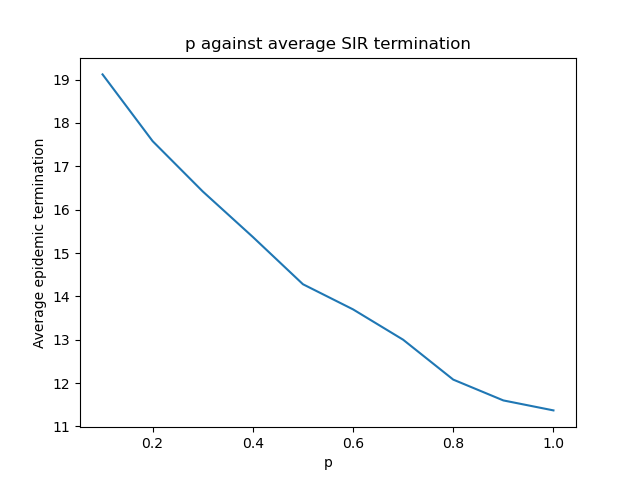
\includegraphics[scale=0.5]{p_sir_t} & 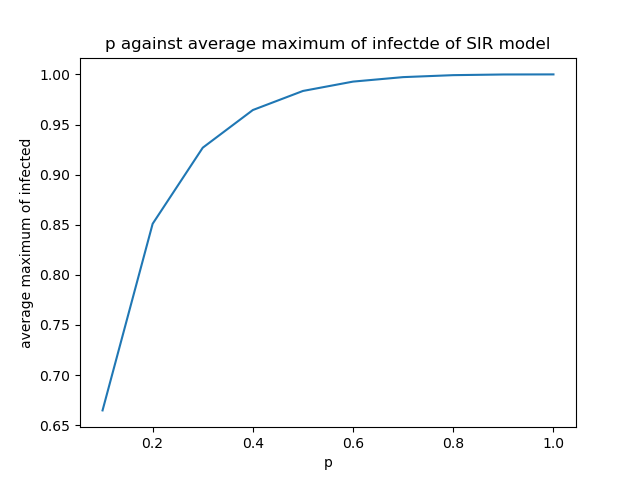
\includegraphics[scale=0.5]{p_infect_sir}\\
    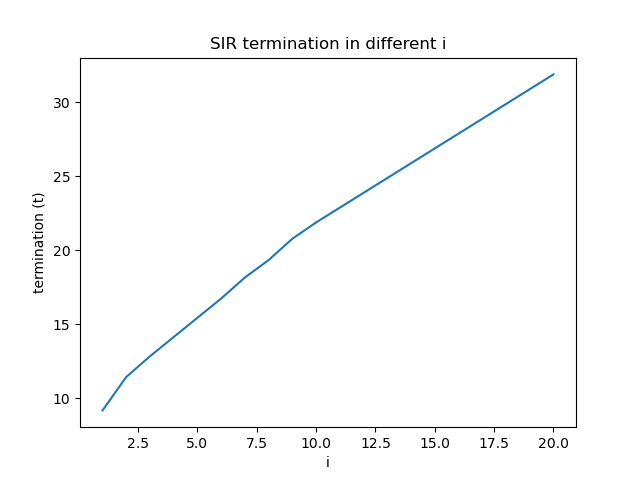
\includegraphics[scale=0.5]{sir_termin_i}&\\
  \end{tabular}

  For \(i\), we can observe that the average termination of the epidemic increases linearly when the length of infectious period increased. The average fraction of infected shows a logarithmic increase also.

  To explain the exponential decay of SIR epidemic termination when \(p\) increased, at each wave \(a\), there will be \(k^a\) contacts. And the expected number of infected will be \(p^a k^a\), which indicates an exponential growth of the number of infected. However, there is finite person in social network, and the infected will not become susceptible again. Without replenish in susceptible, the epidemic is unable to continue to transmit, thus terminates.

  \begin{equation*}
    \sum_{i=1}^a p^i k^i \leq |\text{population in social network}|
  \end{equation*}

  For the logarithmic increase observed when \(p\) or \(i\) increased, it is related to the increase of probability of infection. Firstly, the probability distribution of nodes having \(\geq \alpha\) edges follows an exponential decrease function according to the power law. And a node with more edges connected to has a higher probability of infection of \((1-(1-p)^{|\text{neighbors}|})\). Therefore we can make an assumption that the nodes with more neighbors will be more likly to be infected before the nodes with less neighbors due to a higher probability of infection of the person. This matches the real world scenario of epidemic and the formulation of basic reproduction number. And both changing \(p\) or \(i\) will change the actual probability of infection of the susceptible node in the graph, this can be explained using the function of probability of being not infected \( (1-p)^{i |\text{infected neighbors}|}\). Therefore, in later stage of the epidemic, the susceptible nodes is likly to have few edges, so their actual probability of infection is lower. Thus lead to the logarithmic growth of number of infected.

  For \(s\), we can observe a decreasing trend of termination of epidemic when \(s\) increases, while the number of infected is not affected. Changing the number of initially infected affects the termination of the epidemic only is because it changes the number of infected at the beginning. Moreover, with more nodes infected, we can expect to have more nodes have in-links from the infected nodes. Thus increasing the speed of infection at the beginning phase of the epidemic and therefore the epidemic enters the later phase and terminates faster.

  \subsection{SIRS Model}
  The SIRS model consists of 4 changable parameters \(p, r, i, s\) in the experiment. And the simulations of SIRS epidemic model mostly failed to terminate within 100 waves. Therefore, regression is used to estimate the termination.

  First, on the post-processing of the result, we can observe from the figures of SIRS model simulation (fig. \ref{fig:SIRS1}, \ref{fig:SIRS2}) that there shows a non-linear decreasing trend on the number of maximum infectious nodes in the graph over time. This indicates the drop follows an exponential decreasing function. Thus a logarithm transformation is needed to before fitting the regression line. However, in experiments on the effect of infectious period on the SIRS epidemic model, a linear regression is directly used on the data as the peaks shows a near linear decreasing trend and fitting with \(y = w_1 log(x) + w_0\) exhibit a high error. This is likly to be caused by the increase of \(i\). From the results of SIR model, we can already observe that termination of SIR-modeled epidemics will terminate later when \(i\) increased. The SIR model is similar to a single peak in SIRS infection model. Therefore, with the same magnitude of decrease in number of infected of each peak, but the separation of each peak increased, we can expect the curvature of the function to decrease, thus tends to be a straight line. The increase in the average number of waves between peaks supports the argument. Moreover, when \(i\) increased, the probability of a node not to infect decreases. Therefore, the peak should increase compared to the peaks of smaller \(i\). Therefore, the estimated decreasing function tends to be a straight line when \(i\) is large and the number of iterations is small.

  For SIRS epidemic model, when \(p\) or \(i\) increases, the average maximum fraction of infectious increases following logarithmic increase. The reason is the same as SIR epidemic model, the increase in the probability of infection within a period increases the expected number of nodes of infectious, and the increase in probability affects the nodes with more in-links heavier than those with less in-links. Thus causing the logarithmic increase.

  When \(p\) increases, the predicted termination increases exponentially until \(p=1\). For \(p=1\), the epidemic must transmit to any other susceptible node that the infectious node has outgoing edges to. This causes every node on the graph to be infected stage bt stage. And forms a barrier by the currently infectious and removed nodes for the nodes recovered from removed state back to susceptible state. This can be perceived as a concentric circle, with the center at the initial infectious. The infectious transmit to any nodes it has outgoing edge to, and forms a circular ring of \(i\) width of band of infectious which expands outwards with time. And there is another ring of width \(r\) inside the ring of infectious for the removed nodes. And There is a circle within the ring of removed which are the infected nodes converted back to susceptible according to the SIRS model. Therefore the removed forms a natural barrier or protection to the infected, but now susceptible again nodes. Thus SIRS terminates when \(p=1.0\) in a static social network like in the simulation, but not persists indefinitely like what the basic reproduction number suggests. For \(p<1\), it follows the basic reproduction number, a greater \(p\) may lead to \(R_0>1\), indicating the epidemic may persists with a probability greater than 0. With infection probability less than 1, there may exists susceptible nodes providing as a bridge between the infectious ring and the susceptible circle in the model mentioned previously, allowing the epidemic to persists with oscillation in the number of infectious. And the termination increases exponentially when \(p\) increases, is because with the infection probability increased, it would be harder for a node to not get infected, thus increasing the probability the epidemic to start another wave of infection within the strongly connected social network when many of the nodes have get infected, but converted back to susceptible after \(i+r\) steps.

  When \(i\) increases, average maximum fraction of infectious increases. And the increase follows logarithmic growth. When \(i\) increases, the width of the ring of infectious increases, but as \(i\) increases in an finite graph, the probability of overlap of these rings from different initial infectious increases. Thus the increase of average maximum fraction of infectious decreases when \(i\) increases. And from the data of \(1\leq i \leq 3\), we can observe an exponential growth in the termination of the epidemic. As \(i\) increases, the probability for a node to get infected increases. Therefore we can expect there is a higher chance for the epidemic to persists longer.

  When \(s\) increases, the predicted termination of the epidemic fluctuates. Combining this observation with the average maximum fraction of infectious, I believe change in number of initially infected will not affect the SIRS epidemic in terms of termination. \(s\) increases may speed up the transmission of the epidemic in the beginning stage, but it will not affect the epidemic other than decreasing the time where the first peak of infectious comes.

  For \(r\), from the observation, when \(r\) is large enough, the SIRS epidemic terminates. This shows that \(r\) is inversly proportional to the termination of the epidemic. And increase in \(r\) can effectively increase the number of steps between each peak of infectious in the social network. This can be explained as increasing the width of the barrier between infectious nodes and the susceptible nodes that are recovered from the epidemic using the model mentioned in the explanation of \(p=1\).

  And from observation, the average number of waves between the peaks of infectious in SIRS model is \(i+r+1\). The \(i+r\) part is because of the time needed for the infectious nodes to recover and convert back to susceptible state. While the 1 may be a constant of the time needed for re-transmission in this social network graph.

  \subsection{SIS Model}
  The SIS model is another commonly discussed model like the SIR model. The nodes recovered from the epidemic will be in susceptible state again without immunity to the epidemic. Thus it is more likly for the SIS epidemic model to persist indefinitely. And execpt that SIS model has no Removed state, the mecahnism of SIS model and SIRS model are highly similar. Therefore except for special reasons, the explanations will be referred to the suitable explanation in SIRS.

  From the simulation results, when \(p\) increases, the predicted termination of the epidemic generally increases. This is because when the infection probability increases, it is less likly for the epidemic to cease as the probability of a node to not get transmitted is low. And the average maximum fraction of infectious increases exponentially with a ratio similar to that of the SIRS epidemic simulation. The reason of that is the same as explained in the part explaining the interaction of \(p\) and SIRS execpt that there is no removed state nodes forming a barrier from the susceptible nodes. And the epidemic persists when \(p=1\) in SIS model as there is no removed nodes blocking the re-transmission of the epidemic.

  For \(i\), as stated in SIRS model analysis, when \(i\) increases, the curvature of the decreasing function of the peaks in SIS model decreases, causing the curve tends to be a linear line when \(i\) is large and the number of iterations is small. And the logarithmic increase of average maximum fraction of infectious is explained in SIRS.

  For \(s\), in \(2\leq i \leq 10\), it shows a similar perdicted termination. However, when \(i=1\), the predicted value of termination of the SIS simulation is typically smaller, but the processed simulation data are highly uniform except for 1 outlier.\\
  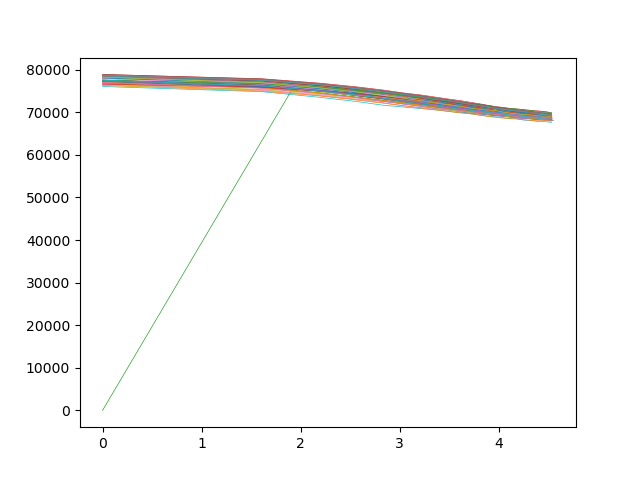
\includegraphics{sis_s1_processed}
  \begin{figure}[!h]
    \caption{Log transformed SIS simulation data of \(s=1\)}
  \end{figure}\\
  Therefore, the difference on termination between \(i=1\) and \(i=2\) might be exhibiting a positive relationship between the number of initially infected and the termination of the epidemic. And the positive relationship might be due to the property of having no removed state in SIS model to block the transmission and allowing the node removed from infectious state to be converted back to infectious in the next step. Thus the increase of intially infected increases the stability and efficiency of the transmission in the graph, and helps in increasing the termination of the epidemic.

  \subsection{Effect of Network Structure on Epidemic}
  With half of the edges randomly removed from the graph, the 90\% effective diameter increased from 4.688472 to 5.024003 while the size of the strongly connected component decreased from 0.86782 to 0.505501. This made the network sparser than the original network and with the distance between nodes increased.

  We can observe a smaller predicted termination and a smaller average maximum fraction of infectious in the SIRS simulation with \(p=0.7, i=3, r=1, s=3\). This demonstrates the effect of connectedness and average distance of the graph on the epidemic. With a higher average distance between the nodes and a smaller strongly connected component, the epidemic is harder to transmit, causing a shorter period will be needed for the epidemic to terminate and less people will be infected. This demonstrates the effect of quarantine and the current ``social distancing'' where people stays at home and connect to each other via the internet instead of having physical social contacts, which with these measures, the edge between people decreases and the size of strongly connected component shrinks. And when these properties of the network decreases, the epidemic terminates faster as the number of contacts decreases, so as the basic reproduction number. Thus showing the effectivness of these measures and the relationship of distance and connectedness of the graph and the epidemic.

  \subsection{Conclusion}
  In conclusion, both infection probability and length period of infectious have huge effect on the three epidemic models. And the number of initial infected have less significant effect to the epidemic models. And change in length of period of removed helps to terminate the epidemic earlier, and bring a termination to the epidemic through quarantine. And the connectedness and the distance between the nodes can also affect the transmission of the epidemic. Thus showing the importance of ``social distancing'' and staying at home in the time when an epidemic occurs epidemics.
\end{document}
